% Chapter 1

\chapter{Introduction} % Main chapter title

\label{Chapter1} % For referencing the chapter elsewhere, use \ref{Chapter1} 

%----------------------------------------------------------------------------------------

% Define some commands to keep the formatting separated from the content 
\newcommand{\keyword}[1]{\textbf{#1}}
\newcommand{\tabhead}[1]{\textbf{#1}}
\newcommand{\code}[1]{\texttt{#1}}
\newcommand{\file}[1]{\texttt{\bfseries#1}}
\newcommand{\option}[1]{\texttt{\itshape#1}}

\newcommand{\mfg}{manufacturer}
\newcommand{\gls}{}

\section{Goals}

%----------------------------------------------------------------------------------------

\section{Methods}

%----------------------------------------------------------------------------------------

\section{Safety-critical devices}
\subsection{What are safety-critical devices?}
% TODO Maybe already mention real-time requirements
The failure or malfunction of a safety-critical system has the potential to cause one or more of the following outcomes:
\begin{itemize}
\item injury or death
\item damage to property
\item environmental harm
\end{itemize}
A safety-critical device is consequently an embedded device with a dedicated function that has the above mentioned property. Such a device always contains electronic hardware but may also have mechanical and/or software components.

% TODO Verify that that is actually part of IEC-61508
The legal entity responsible for designing and manufacturing the device will be referred to as \mfg{}, to stay consistent with IEC-61508. 
\subsection{Basic concepts}
\subsubsection{Safety regulations}
% REWRITE Sounds a bit bad
The main goal of safety-critical device manufacturers is to create a safe device. This protects them from expensive lawsuits and can give them a competitive advantage.

% TODO Think about more commonalities and maybe refactor this
However, in most markets, a favourable real-world safety alone is not enough to gain permission to sell the device.  Each market (medical, nuclear, aviation etc.) and regulatory body (EU, US etc.) has their own standard for normative safety that needs to be met. This thesis will lean mostly on IEC 61508 \cite{IEC.2010-1}\cite{IEC.2010-2}\cite{IEC.2010-3} because it represents a general standard from which many others derive. And although there are important differences that need to be kept in mind, for the purpose of this thesis the standards are similar enough to be interchangeable. [source or further justification?]

The specific instructions and required level of rigour differ between the standards but they usually share the following requirements:

\begin{itemize}
\item A compliant quality management system needs to be used
\item Device requirements need to be analyzed
\item Requirements need to be verified
\item Unreasonable risk needs to be reduced
\item Extensive documentation on all aspects of design and manufacturing needs to be created
\end{itemize}

The \mfg{} also has to present the documents that he generated along the way to the authorities. There are exceptions to this rule, if third-party or legacy parts are used but these need to be justified as well. Therefore, it is usually infeasible to certify a device after the development process, if it was not designed with certification in mind. 

A failed certification attempt is undesirable, as it is associated with additional cost and time but it is also not a death sentence for the device. The regulatory body will point out the problems and give the \mfg{} the option to fix them and resubmit the device for certification.

The rigour that is demanded by regulatory bodies is dependent on the risk category that can be assigned to the safety functions of the device. These risk categories will be called \keyword{criticality levels} from here on out. 

\subsubsection{Criticality levels}
% TODO Verify that this is actually all true
% REWRITE 
[Unhappy with how this section is written]
IEC 61508 calls criticality levels \keyword{Safety integrity levels} or  \gls{SIL} for short. The standard defines \keyword{safety integrity} as \textquote{the likelihood of a safety-related system satisfactorily performing the required safety functions under all the stated conditions, within a stated period of time}\cite{IEC.2010-1}. The SIL of a safety function is the target probability of a dangerous failure occurring within a certain time [Table of probabilities is not yet added]. In IEC 61508 there are safety integrity levels from 1 to 4, where SIL 1 is the lowest and SIL 4 the highest. The level basically defines the rigor that is required during the development process.

% TODO Maybe explain the basics of the risk assessment in IEC 61508
Risk assessment is the process that drives the categorization of a system into the safety integrity levels and if the SIL of a system is too high it can be reduced by introducing risk mitigation mechanisms. For example, if the software of a device would be SIL 4 initially, it might be reduced by adding a second processor that runs distinct software, that can verify the validity of the initial software's output.  In fact SIL 4 is considered too high to be feasible and is practically always reduced \cite{MTLInstrumentsGroup.March2002}.

[I will also give an outline of the medical software classes, how they are different, and why the differences aren't really that important for this thesis]

\begin{comment}
\begin{table}[H]
\begin{tabular}{|l|l|l|}
\hline
\textbf{Category} & \textbf{Definition}                & \textbf{Range (failures per year)} \\ \hline
Frequent          & Many times in system lifetime      & >$10^{-3}$                         \\ \hline
Probable          & Several times in system lifetime   & $10^{-3}$ to $10^{-4}$             \\ \hline
Occasional        & Once in system lifetime            & $10^{-4}$ to $10^{-5}$             \\ \hline
Remote            & Unlikely in system lifetime        & $10^{-5}$ to $10^{-6}$             \\ \hline
Improbable        & Very unlikely to occur             & $10^{-6}$ to $10^{-7}$             \\ \hline
Incredible        & Cannot believe that it could occur & >$10^{-7}$                         \\ \hline
\end{tabular}
\caption{Categories of likelihood in IEC-61508}
\label{categories-of-likelihood}
\end{table}

\begin{table}[H]
\begin{tabular}{|l|l|}
\hline
\textbf{Category} & \textbf{Definition}                   \\ \hline
Catastrophic      & Multiple loss of life                 \\ \hline
Critical          & Loss of a single life                 \\ \hline
Marginal          & Major injuries to one or more persons \\ \hline
Negligible        & Minor injuries at worst               \\ \hline
\end{tabular}
\caption{Categories of consequence in IEC-61508}
\label{consequence-categories}
\end{table}

\begin{table}[H]
\begin{tabular}{|l|l|l|l|l|}
\hline
                    & \multicolumn{4}{c|}{\textbf{Consequence}}       \\ \hline
\textbf{Likelihood} & Catastrophic & Critical & Marginal & Negligible \\ \hline
Frequent            & I            & I        & I        & II         \\ \hline
Probable            & I            & I        & II       & III        \\ \hline
Occasional          & I            & II       & III      & III        \\ \hline
Remote              & II           & III      & III      & IV         \\ \hline
Improbable          & III          & III      & IV       & IV         \\ \hline
Incredible          & IV           & IV       & IV       & IV         \\ \hline
\end{tabular}
\caption{Typical risk class matrix for IEC-61508}
\label{risk-class-matrix}
\end{table}

\begin{itemize}
    \item Class I: Unacceptable in any circumstance
    \item Class II: Undesirable: tolerable only if risk reduction is impracticable or if the costs are grossly disproportionate to the improvement gained
    \item Class III: Tolerable if the cost of risk reduction would exceed the improvement
    \item Class IV: Acceptable as it stands, though it may need to be monitored
\end{itemize}
\end{comment}

% NOTE Do I gloss over this point too much? Or should it be mentioned here in the first place?
Other standards define criticality levels differently, but no matter what definition of criticality levels is applied, they all share two properties that motivate the rest of this thesis: First, a function with a higher criticality level is more expensive to implement and verify than one with a lower level. There is more documentation effort, more rigorous risk analysis, verification and validation. 

Second, two units of a device are only allowed to have differing criticality levels, if there is sufficient evidence that the higher criticality function is independent from the lower criticality function \cite{IEC.2010-1}\cite{IEC.2010-2}.  % NOTE Is there something missing here?

% NOTE There is a weird jump from the last section to this one
This constellation of heterogeneous criticality levels within the device is very common and usually referred to as mixed criticality. Its motivations and problems will be explored in the next section.
\subsection{Mixed criticality} \label{mixed-criticality}
\subsubsection{Motivations}
The core motivation for assigning different criticality levels within a device has already been mentioned; it is cheaper to implement and verify a low criticality part. But this is not the only motivation, as it only applies to functionality that is implemented by the \mfg{} and not by a third-party.

% NOTE Get a hardware perspective
Using third-party software can save costs and accelerate time to market. Currently the default is to use pre-certified software that is specifically developed for this purpose. This can limit the problems that mixed criticality entails all together but because of the narrow target audience this kind of software is more expensive and more limited in its functionality. Ideally it would be possible to use regular off-the-shelf software or even free open-source software but as established earlier certifying this software according to a level of criticality is completely infeasible.

In fact, being able to use third-party software unhindered can have even more drastic impacts than saving some money on the certification process. It can make certain functionality, especially in the realm of usability, feasible in the first place. And with the growing consumer demands, even in the safety-critical sector \cite{ITA.May2016}, this can really differentiate a device from the rest of the market.

Now it is clear why mixed criticality is actually a desirable property in a lot of devices. It can save cost and time, as well as provide functionality indirectly that would have been infeasible to realize without.
\subsubsection{Problems}
% NOTE Make sure the point I reiterate here is clearly made in the previous section
As alluded to earlier, mixed criticality does not come without problems. Regulatory standards require sufficient evidence for independence between functions of different criticality be shown to them \cite{IEC.2010-1}\cite{IEC.2010-2}. If \mfg{} can not provide this evidence all functions need to comply to the highest criticality level.

Sufficient independence is given, if it can be shown that a dependent failure between the higher and lower criticality function is sufficiently low in the context of the highest level.
To achieve this a system architecture is required that can reliably separate components. The precise requirements this separation architecture needs to fulfill will be tackled in the next section.

%----------------------------------------------------------------------------------------

\section{The separation architecture} \label{separation-arch}
% TODO Cite Wittenstein white papers
% NOTE Think about where and how to mention real-time requirements
There are four attributes the separation architecture needs to solve the mixed criticality problem.
\subsection{Spatial separation}

\begin{comment}
\begin{figure}
\centering
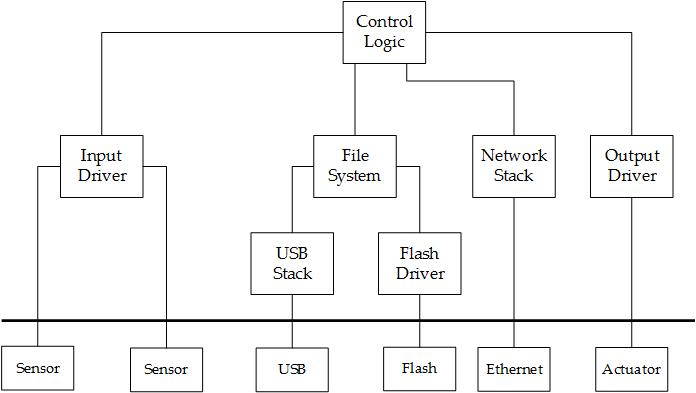
\includegraphics{Figures/Drawing1}
\decoRule
\caption{Test}
\label{fig:sepArch}
\end{figure}
\end{comment}

Spatial separation means that access of physical resources cannot lead to conflicts or corruption. This includes memory access as well as system resources such as hardware peripherals. \cite{Wittenstein.spatial.2017}\cite{perez2013safety}

If shared access to any system resources is necessary, some kind of arbiter needs to be in place to give consistent access to components based on their criticality. 
\subsection{Temporal separation}
Temporal separation is achieved, if it is sufficiently unlikely for any system software to compromise the processing demands of another \cite{Wittenstein.temporal.2017}. 
Managing access to available processing resources is the main part of temporal separation. However, system events and triggers may also require analysis. Excessive interrupt routine run time, for example, can cause processing resources to be unavailable to the main system \cite{Wittenstein.temporal.2017}. 
\subsection{Data integrity and validity}
Data passed through unsafe components has to be either not safety related or protected. Whereas protection refers to ensuring the data's integrity and validity after it has passed through the unsafe components and before it is used in safety related processing \cite{Wittenstein.spatial.2017}.

In practice this requirement doesn't have to be met by the architecture but may be handled in the application software. Nevertheless it is an important aspect that needs to be kept in mind.
\subsection{Certifiable compliance}
It may not come as a surprise that the separation architecture also needs to fulfill these requirements in the eyes of the regulatory bodies, as they are the reason for the architecture's inception.
How this may be achieved differs based on architecture and standard but it needs to be feasible at the very least. 

%----------------------------------------------------------------------------------------

\section{Existing architectures}
% TODO Refrain from comparing architectures (or even making qualitative judgments) unless I am building the argument for not analyzing them later. Or I guess only talk about quality of separation (more sources!)
\subsection{Embedded operating systems}
% NOTE There is a gap between this section and the previous
Apart from bare-metal software, which is reserved for the most trivial cases,  embedded operating systems are the simplest approach to device architecture. 
% NOTE Feels like there is also something missing here
\subsubsection{General purpose operating system}
Even though this section's title is \keyword{General purpose operating system} (GPOS) realistically it can be substituted with Linux, as other options are usually not considered adequate for embedded devices. But the same arguments should apply to other general purpose operating systems.

With the help of an \gls{MMU} or \gls{MPU}  a \gls{GPOS} can achieve the spatial separation of memory between applications. The operating system's access control can be used to limit peripheral access and drivers can arbitrate conflicts. 

% NOTE Am i confusing temporal separation with being able to satisfy real-time requirements?
Temporal separation is usually not possible and may even be counter-productive to the standard processing model of general purpose operating systems, since they are designed to optimize average case performance and sacrifice determinism for it. There are however ongoing efforts to introduce temporal separation as well as the ability to reliably satisfy real-time requirements into the Linux kernel \cite{SiroArthur.2007}.
[I might have confused temporal separation with being able to satisfy real-time requirements in the preceding section]

% REWRITE This section is a bit strange
Undoubtedly these efforts have been at least somewhat successful as Linux has been successfully deployed in some safety-critical systems with hard real-time requirements. One big issue remains however, Linux is massive with several millions lines of code and safety can only be reasoned about on the basis of its "proven in use" status [Maybe mention Roche Linux as a counter example]. This is not enough for most regulatory bodies, especially in devices with high criticality, where the benefits of mixed criticality are the most pronounced.

Another big problem is damage limitation. While more and more Linux drivers are implemented in user space, a considerable amount still has to be in kernel space [Point could be stronger]. Failures in these drivers can potentially cause a kernel panic, prompting the device to shut down. 

Perhaps Linux, or another, yet unknown GPOS, will be able to solve the mixed criticality problem directly but for now it will be excluded from further analysis, on the grounds that it can not satisfy the separation architecture requirements well enough for a large set of safety-critical devices.
\subsubsection{Real-time operating system}
% NOTE How do they deal with peripherals?
Providing temporal separation is practically the main purpose of an RTOS, so there are no real problems on that front, and with the aid of an \gls{MPU} or \gls{MMU} spatial separation is also not a big issue.

One thing to keep in mind though is that a lot of RTOS developers offer no multicore support, which can severely limit the complexity of an application. But perhaps the biggest limitation of application complexity on the RTOS architecture is its narrow target audience.

As a result of this, there is a distinct lack of sophisticated middleware [source?]. Especially cutting edge usability technology, like touch gesture recognition, is likely not available on these platforms. At the same time consumers are becoming increasingly adept at recognizing good design and are demanding strong user interfaces \cite{HBR.September2015}.
Additionally, a problem outlined in the section \ref{mixed-criticality} applies to RTOS middleware as well: These libraries have a similarly narrow target audience and can therefore be quite expensive for the functionality they offer.

Although the RTOS architecture remains quite a dominant one, it quickly loses its appeal with growing application complexity. Therefore it will be excluded from further analysis in this thesis.
\subsection{AMP / Multicore system}
More and more silicon vendors are offering multicore systems with a dedicated safety and a support core. These are usually heterogeneous processors with one application core, like an ARM Cortex A7, and one microcontroller core, like an ARM Cortex M4. Proving temporal separation on these systems is typically not difficult, as the cores are physically separated \cite{Wittenstein.temporal.2017}.

But the cores in these systems share hardware resources like peripherals and memory. Consequently, it can be challenging to show sufficient evidence for spatial separation. An \gls{MMU} or \gls{MPU} can be useful to enforce spatial separation but it is not a perfect solution, especially for peripherals [Why?]. 
\subsection{Hardware supervised AMP / Hardware supervised Multicore system}
These systems are identical to the ones described in the previous section, except they contain additional hardware to control and arbitrate peripheral access, as well as inter-core communication.
Because there is no standard for this, the implementation is entirely up to the silicon vendor. 

Although this hardware supervision has limited functionality, it has a clear advantage over comparable software solutions, like a hypervisor: Hardware is less error prone than software and this is recognized by regulatory bodies, in the form that software has to adhere to much stricter rules \cite{IEC.2010-3}. It is therefore possible that these systems are cheaper than hypervisors overall. 

This architecture should be considered when designing a safety-critical device but it is still fairly new and a full analysis of it is not in the scope of this thesis.
\subsection{Hardware separated subsystems / Multiprocessor system}
% NOTE review http://www.ia.pw.edu.pl/~tkruk/edu/eopsya/lecture/eopsy08.pdf and http://www-5.unipv.it/mferretti/cdol/aca/Charts/07-multiprocessors-MF.pdf and if these are viable
% TODO https://witekio.com/blog/introduction-heterogeneous-multicore-processing-architecture/ Read about the need for software support on this architecture
% TODO actually explain what they are
Multiprocessor systems or even completely separate subsystems are the current status quo for dealing with the mixed criticality problem. The multiprocessor architecture should not be confused with the multicore architecture, as it has distinct processors, usually with their own resources, on the same or different \gls{PCB}s.

Such a system starts out with perfect temporal and spatial separation because the systems are fully independent. The \mfg{} can then reintroduce dependence in very deliberate and controlled ways, that don't impact the device's safety rating. For example by introducing a dedicated communication channel between the processors. 

% NOTE Is this a qualitative assessment better reserved for the analysis part?
Keep in mind however that, while sharing external peripherals is theoretically possible, it is not commonly done and poses some difficult concurrency challenges. This means that any external peripheral that could theoretically be shared has to be duplicated instead. The same goes for memory.

More specific advantages and disadvantages of this architecture will be analyzed in more detail later in the thesis.

%----------------------------------------------------------------------------------------

\section{Embedded safety hypervisor origins}
% TODO Add dat sauce
Now let's examine the main subject of analysis, the embedded safety hypervisor. In this section it will be established where it comes from and some basic associated concepts. This should get rid of some common misconceptions about hypervisors and their applicability in the embedded sector.
\subsection{Hardware virtualization} \label{hw-virt}
The act of \keyword{hardware virtualization} refers to the creation of a virtual machine  that acts exactly like a real device. Software executed on this machine has no direct access to the underlying hardware resources. Virtual machines are typically called guests, whereas the device virtualizing them is referred to as the host machine
There are two types of \keyword{hardware virtualization}.
\paragraph{Para-virtualization}
Para-virtualized guests run in a separated environment with no direct access to the hardware but their hardware environment is not simulated. That means guest software needs to be modified to run in this environment.
\paragraph{Full virtualization}
In full virtualization the entire guest hardware is simulated, allowing guest software to run completely unmodified.

Doing this kind of simulation entirely in software is very computationally expensive and has only really become feasible with hardware virtualization extensions. These virtualization extensions add an additional level of privilege to the processor, along with additional instructions and hardware enhancements that make virtualization a lot more efficient \cite{ARM.v8.2018}.

Notably, while these extensions where originally limited to high powered hardware, they have since become available in more embedded focused processor lines like the Intel Atom and ARMv7/v8.
\subsection{Original hypervisor use case}
Hypervisors were originally conceived in the 1960s as a way of accommodating multiple users on mainframe computers. After a hiatus they enjoyed their resurgence in the 2000s when the demand on servers rose again. 

So they started out as a way to maximize resource utilization in large servers. However, low resource utilization is usually not an issue in embedded systems, quite the opposite in fact. Therefore these original hypervisors are not the point of discussion for this thesis.
\subsection{Microkernels}
At this point it is useful to make a quick excursion to the realm of microkernels. As the name implies their guiding principal is that of minimal trusted computing base. Basically everything that doesn't absolutely have to be handled in kernel space for the device to work is implemented in user space.

This kind of system was exclusive to academia for a long time, until it somewhat matured in the late 90s \cite{Liedtke.1995}\cite{Liedtke.1996}. With this development they had already become attractive to safety-critical device manufacturers and saw some large scale deployment.

\subsection{Unification of the two concepts}
In 2005 an academic debate broke out about the legitimacy of microkernels versus the hypervisors that were around at this time. 
The argument was that, despite their architectural similarities, hypervisors are a special case of microkernels \textquote{microkernels done right} \cite{StevenHand.2005}\cite{Heiser.2006}. Without examining the back and forth that ensued, the result was the addition of hypervisor functionality to existing microkernels \cite{Heiser.2010}. And these hypervisors with a minimal trusted computing base were focused on the safety-critical market, providing safe separation instead of maximum resource utilization.

This does not necessarily mean that microkernel based hypervisors are the definitive embedded safety hypervisor but it is their origin and still by far the most prevalent architecture.


